\begin{figure}
\begin{center}
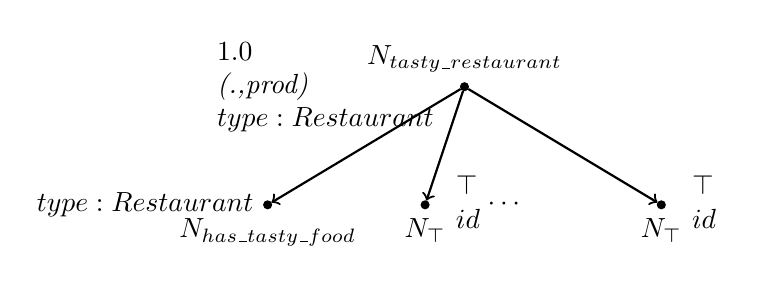
\begin{tikzpicture}[yscale=-1,
place/.style={circle,draw=black, fill=black, inner sep=0pt, 
              minimum size=1mm}]

  \node[place] (1st) at (2.5, 0) [label=above: $N_{tasty\_restaurant}$,
                                label=left: 
             \begin{tabular}{l}
               $1.0$\\
               \textit{(.,prod)}\\
               $type : Restaurant$\\
             \end{tabular}
] {};
	\node[place] (2nd) at (0, 1.5) [label=below: $N_{has\_tasty\_food}$, 
        label=left: $type : Restaurant$] {};
        \node[place] (3rd) at (2, 1.5) [label=below: $N_{\top}$,
          						  label=right: 
             \begin{tabular}{l}
            $\top$\\
            $id$\\
             \end{tabular}
             ] {}; 
        \node[place] (4rd) at (5, 1.5) [label=below: $N_{\top}$,
          						  label=right: 
             \begin{tabular}{l}
            $\top$\\
            $id$\\
             \end{tabular}
             ] {}; 

        \node (dots) at (3,1.5) {$\cdots$};
	
	\draw[->, thick] (1st) -- (2nd);
        \draw[->, thick] (1st) -- (3rd);
        \draw[->, thick] (1st) -- (4rd);
\end{tikzpicture}
\end{center}   
\caption{predicate tree for tasty\_restaurant with equivalence extension}
\label{fig:ex2.2}
\end{figure}